% Étape 3 (2/2) : multi-têtes, recoller, résiduel, MLP — matrices + tableau
% (suite du tableau 1/2, même style). Compiler avec pdflatex (ou Overleaf).
\documentclass[border=10pt,varwidth=760pt]{standalone}
\usepackage[T1]{fontenc}
\usepackage[utf8]{inputenc}
\usepackage[scaled]{helvet}
\renewcommand{\familydefault}{\sfdefault}
\usepackage{sansmath}
\sansmath
\usepackage{amsmath}
\usepackage{array}
\usepackage{xcolor}
\usepackage{colortbl}
\usepackage{tikz}
\usetikzlibrary{arrows.meta}

\definecolor{orange}{HTML}{FFD0BF}
\definecolor{creme}{HTML}{FFF6EC}
\definecolor{jaune}{HTML}{FFE2A8}
\definecolor{rose}{HTML}{FFC2C8}
\definecolor{tA}{HTML}{FFE2A8}
\definecolor{tB}{HTML}{FFC2C8}
\definecolor{tC}{HTML}{FFB8A0}
\definecolor{tD}{HTML}{F3D6E6}
\definecolor{bordeaux}{HTML}{3F161C}

\newcommand{\num}[1]{\textbf{#1}}
\renewcommand{\arraystretch}{2.1}
\arrayrulecolor{orange}

\tikzset{
  t/.style={font=\fontsize{13}{15}\selectfont, text=black, inner sep=0pt},
  ts/.style={font=\fontsize{12}{14}\selectfont, text=black, inner sep=0pt},
  op/.style={font=\fontsize{16}{18}\selectfont, text=black, inner sep=0pt},
  fl/.style={bordeaux, line width=1.4pt, -{Stealth[length=7pt]}},
}
\newcommand{\grid}[6]{%
  \fill[#6] (#1,#2) rectangle ++(#4*#5,#3*#5);
  \ifnum#4>1 \foreach \k in {1,...,\numexpr#4-1\relax} \draw[white, line width=1pt] (#1+\k*#5,#2) -- ++(0,#3*#5); \fi
  \ifnum#3>1 \foreach \k in {1,...,\numexpr#3-1\relax} \draw[white, line width=1pt] (#1,#2+\k*#5) -- ++(#4*#5,0); \fi}
\newcommand{\tetes}[3]{%
  \grid{#1}{#2}{4}{2}{#3}{tA} \grid{#1+2*#3}{#2}{4}{2}{#3}{tB}
  \grid{#1+4*#3}{#2}{4}{2}{#3}{tC} \grid{#1+6*#3}{#2}{4}{2}{#3}{tD}
  \foreach \k in {1,2,3} \draw[white, line width=2.5pt] (#1+2*\k*#3,#2) -- ++(0,4*#3);}

\begin{document}
\fontsize{13}{16}\selectfont

% ---------------- matrices ----------------
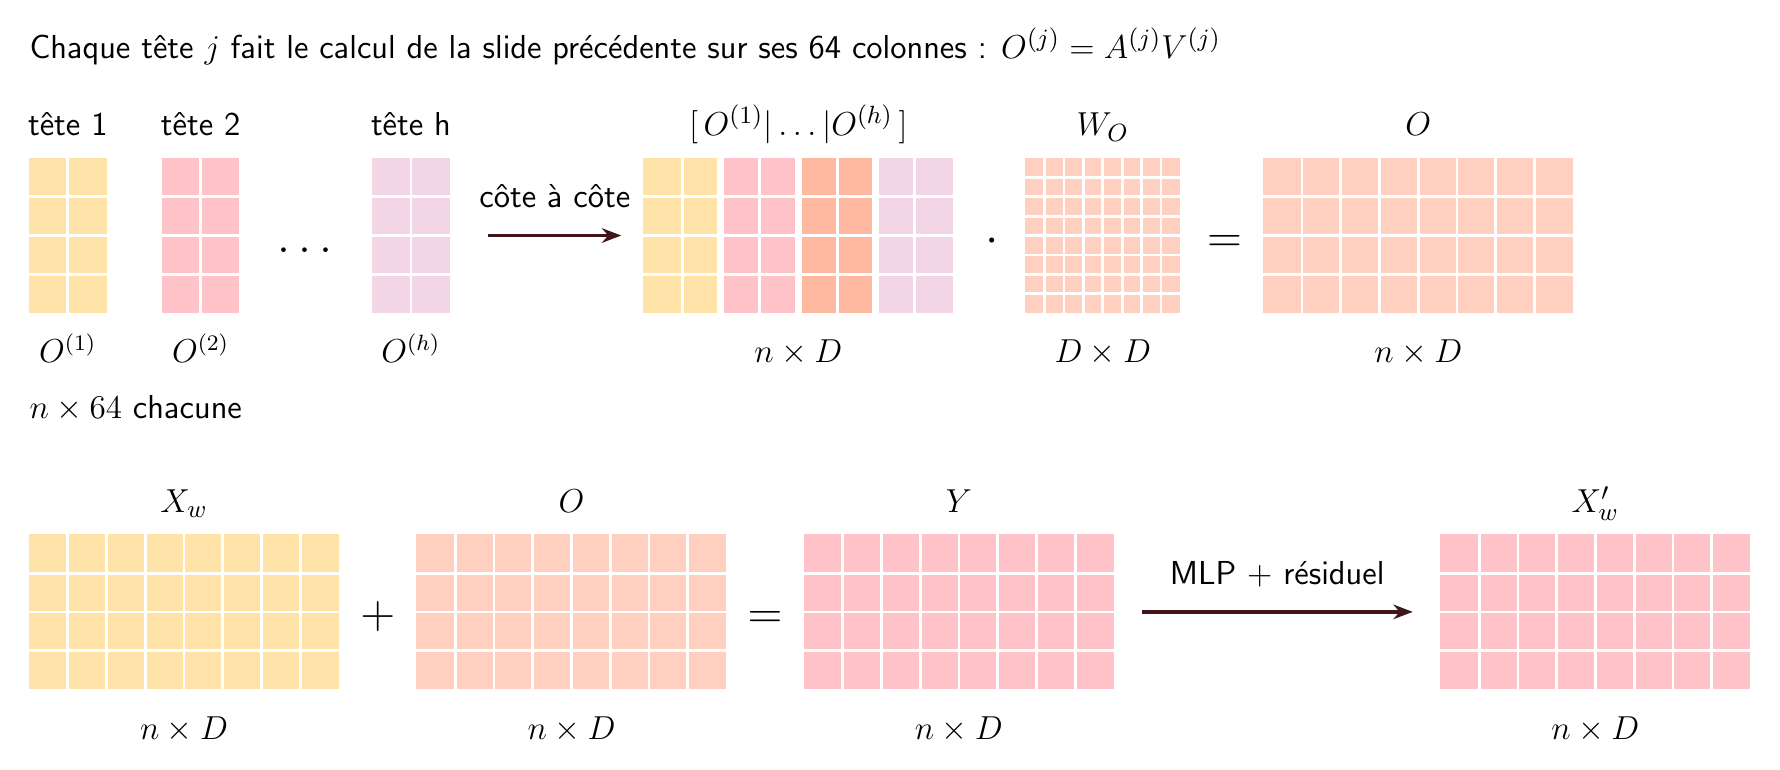
\begin{tikzpicture}[x=1pt, y=-1pt, line join=miter]
% ligne 1 : les h têtes -> recollées -> . W_O = O
\node[t, anchor=base west] at (0,0) {Chaque tête $j$ fait le calcul de la slide précédente sur ses 64 colonnes : $O^{(j)} = A^{(j)} V^{(j)}$};
\foreach \j/\c/\x in {1/tA/0, 2/tB/48, h/tD/124} {
  \node[ts, anchor=base] at (\x+14,28) {tête \j};
  \grid{\x}{36}{4}{2}{14}{\c}
  \node[ts, anchor=base] at (\x+14,110) {$O^{(\j)}$};
}
\node[op, anchor=base] at (101,70) {$\dots$};
\node[ts, anchor=base west] at (0,130) {$n \times 64$ chacune};

\draw[fl] (166,64) -- (214,64);
\node[ts, anchor=base] at (190,54) {côte à côte};
\node[t, anchor=base] at (278,28) {$[\,O^{(1)} | \dots | O^{(h)}\,]$};
\tetes{222}{36}{14}
\node[op, anchor=base] at (348,70) {$\cdot$};
\node[t, anchor=base] at (388,28) {$W_O$};
\grid{360}{36}{8}{8}{7}{orange}
\node[op, anchor=base] at (432,70) {$=$};
\node[t, anchor=base] at (502,28) {$O$};
\grid{446}{36}{4}{8}{14}{orange}
\node[ts, anchor=base] at (278,110) {$n \times D$};
\node[ts, anchor=base] at (388,110) {$D \times D$};
\node[ts, anchor=base] at (502,110) {$n \times D$};

% ligne 2 : résiduel puis MLP
\node[t, anchor=base] at (56,164) {$X_w$};
\grid{0}{172}{4}{8}{14}{jaune}
\node[op, anchor=base] at (126,206) {$+$};
\node[t, anchor=base] at (196,164) {$O$};
\grid{140}{172}{4}{8}{14}{orange}
\node[op, anchor=base] at (266,206) {$=$};
\node[t, anchor=base] at (336,164) {$Y$};
\grid{280}{172}{4}{8}{14}{rose}
\draw[fl] (402,200) -- (500,200);
\node[ts, anchor=base] at (451,190) {MLP + résiduel};
\node[t, anchor=base] at (566,164) {$X'_w$};
\grid{510}{172}{4}{8}{14}{rose}
\node[ts, anchor=base] at (56,246) {$n \times D$};
\node[ts, anchor=base] at (196,246) {$n \times D$};
\node[ts, anchor=base] at (336,246) {$n \times D$};
\node[ts, anchor=base] at (566,246) {$n \times D$};
\end{tikzpicture}

\vspace{14pt}

% ---------------- tableau (suite du 1/2) ----------------
\begin{tabular}{>{\centering\arraybackslash}m{22pt} >{\raggedright\arraybackslash}m{95pt} >{\raggedright\arraybackslash}m{250pt} >{\centering\arraybackslash}m{62pt} >{\raggedright\arraybackslash}m{268pt}}
\rowcolor{creme}
 & \textbf{Étape} & \textbf{Formule} & \textbf{Taille} & \textbf{Ce que ça fait} \\
\hline
\num{6} & Têtes & $Q = [\,Q^{(1)} | \dots | Q^{(h)}\,]$ (idem $K, V$), $h = D/64$ & $n \times 64$ & les étapes 3 à 5 faites $h$ fois, en parallèle \\
\hline
\num{7} & RoPE & $Q^{(j)}, K^{(j)}$ tournés selon la position & $n \times 64$ & le score dépend de la distance entre patchs \\
\hline
\num{8} & Recoller & $O = [\,O^{(1)} | \dots | O^{(h)}\,]\, W_O$ & $n \times D$ & on rassemble les $h$ têtes ($h \times 64 = D$) \\
\hline
\num{9} & Résiduel & $Y = X_w + O$ & $n \times D$ & on ajoute une correction, sans tout remplacer \\
\hline
\num{10} & MLP & $X'_w = Y + \mathrm{GELU}\big(\mathrm{Norm}(Y)\, W_1\big)\, W_2$ & $n \times D$ & chaque patch est transformé seul ($D \rightarrow 4D \rightarrow D$) \\
\hline
\end{tabular}

\vspace{10pt}
{\fontsize{12}{15}\selectfont
$W_O$ : $D \times D$ \qquad $W_1$ : $D \times 4D$ \qquad $W_2$ : $4D \times D$ \qquad (appris) \qquad $h$ = 4 (S), 6 (M), 8 (L)

\vspace{4pt}
Entrée $X_w$ : $n \times D$ \ $\rightarrow$ \ Sortie $X'_w$ : $n \times D$ (même taille) \ $\rightarrow$ les 16 fenêtres sont recollées, puis Swin\par}
\end{document}
